\section{\textlatin{UI/UX}}
Η σχεδίαση του \textlatin{UI/UX} έγινε έτσι ώστε ο χρήστης, δηλαδή ο μαθητής που θα μπει στην σελίδα, να μπορεί να πλοηγείται με ευκολία και οργάνωση, προκειμένου να μπορεί να βοηθηθεί εν συνεχεία και στην απόδοσή του στα μαθήματα. Η πλοήγηση του μαθητή θα γίνεται σειριακά. Συγκεκριμένα:

\begin{itemize}
    \item Ο μαθητής θα αρχίζει κάνοντας \textbf{\textlatin{Login}} στην αρχική φόρμα που θα του εμφανίζεται (την πρώτη φορά που θα επισκεφτεί την σελίδα θα πρέπει να δημιουργήσει τον λογαριασμό του χρησιμοποιώντας την αντίστοιχη φόρμα \textbf{\textlatin{Register}}.
\end{itemize}
\begin{figure}[H]
        \centering
        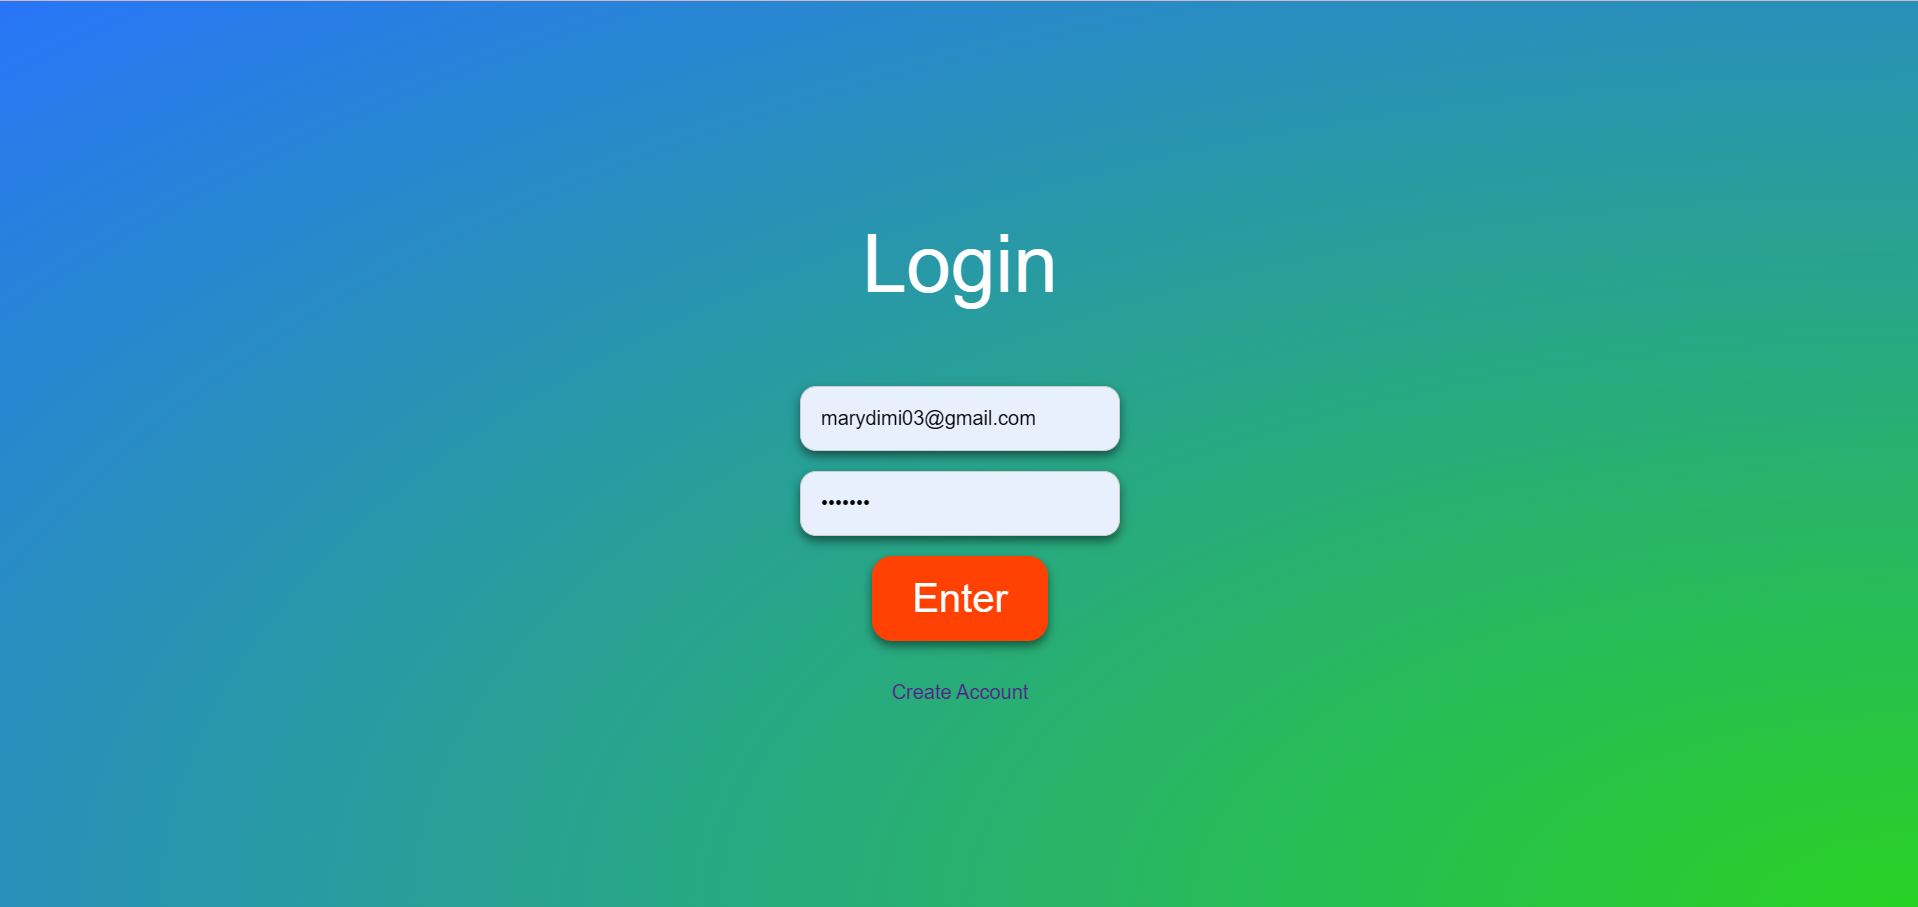
\includegraphics[width=1\linewidth]{img/Login.png}
        \caption{\textlatin{Login Page}}
\end{figure}
\begin{figure}[H]
    \centering
    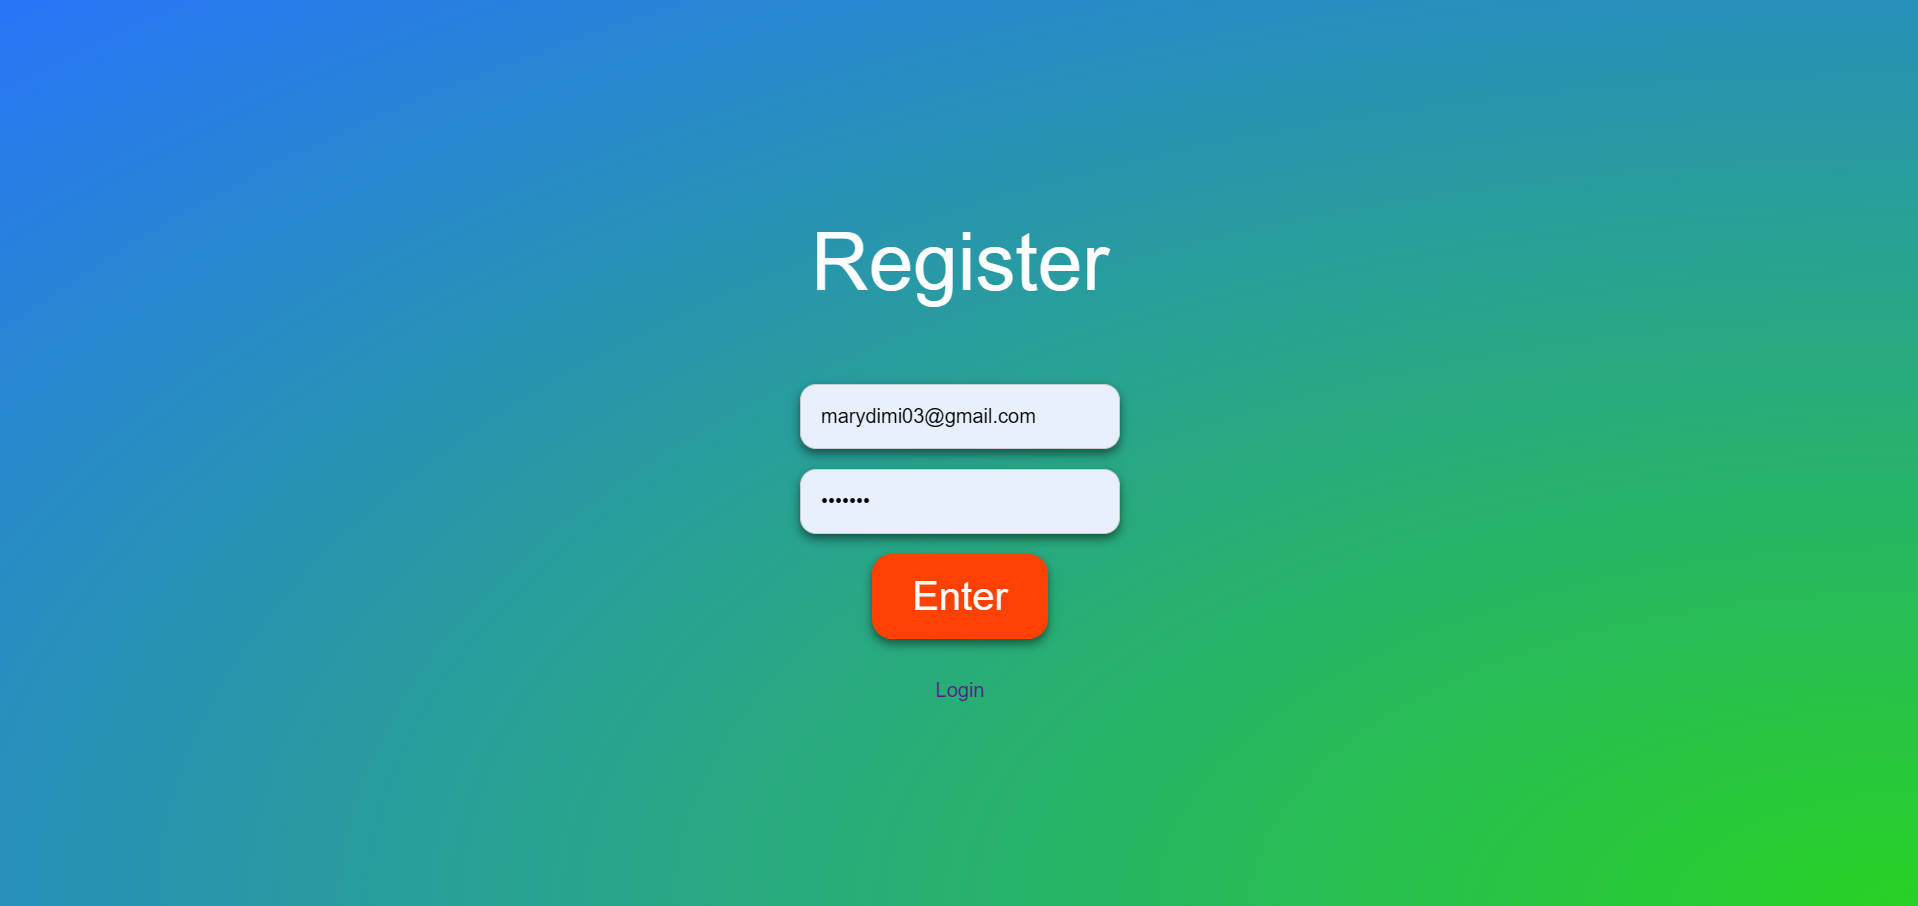
\includegraphics[width=1\linewidth]{img/Register.png}
    \caption{\textlatin{Register Page}}
\end{figure}

\begin{itemize}
    \item Στην συνέχεια θα ακολουθεί το \textbf{κεντρικό μενού,} με τις επιλογές να αρχίσει ή να συνεχίσει την πρόοδο του (\textbf{\textlatin{Learn/Continue}}), εφόσον το λογισμικό θα "θυμάται" που έχει μείνει ο κάθε μαθητής, θα μπορεί να προσπελάσει την λίστα όπου θα φαίνονται όλα τα διαθέσιμα κεφάλαια (\textlatin{\textbf{Chapters}}) και η τελευταία θα είναι να δει τα στατιστικά του (\textbf{\textlatin{Statistics}}), δηλαδή με πιο απλά λόγια τις επιδόσεις του στις δραστηριότητες που έχει ολοκληρώσει (\textlatin{quizzes, exam}).
\end{itemize}
\begin{figure}[H]
    \centering
    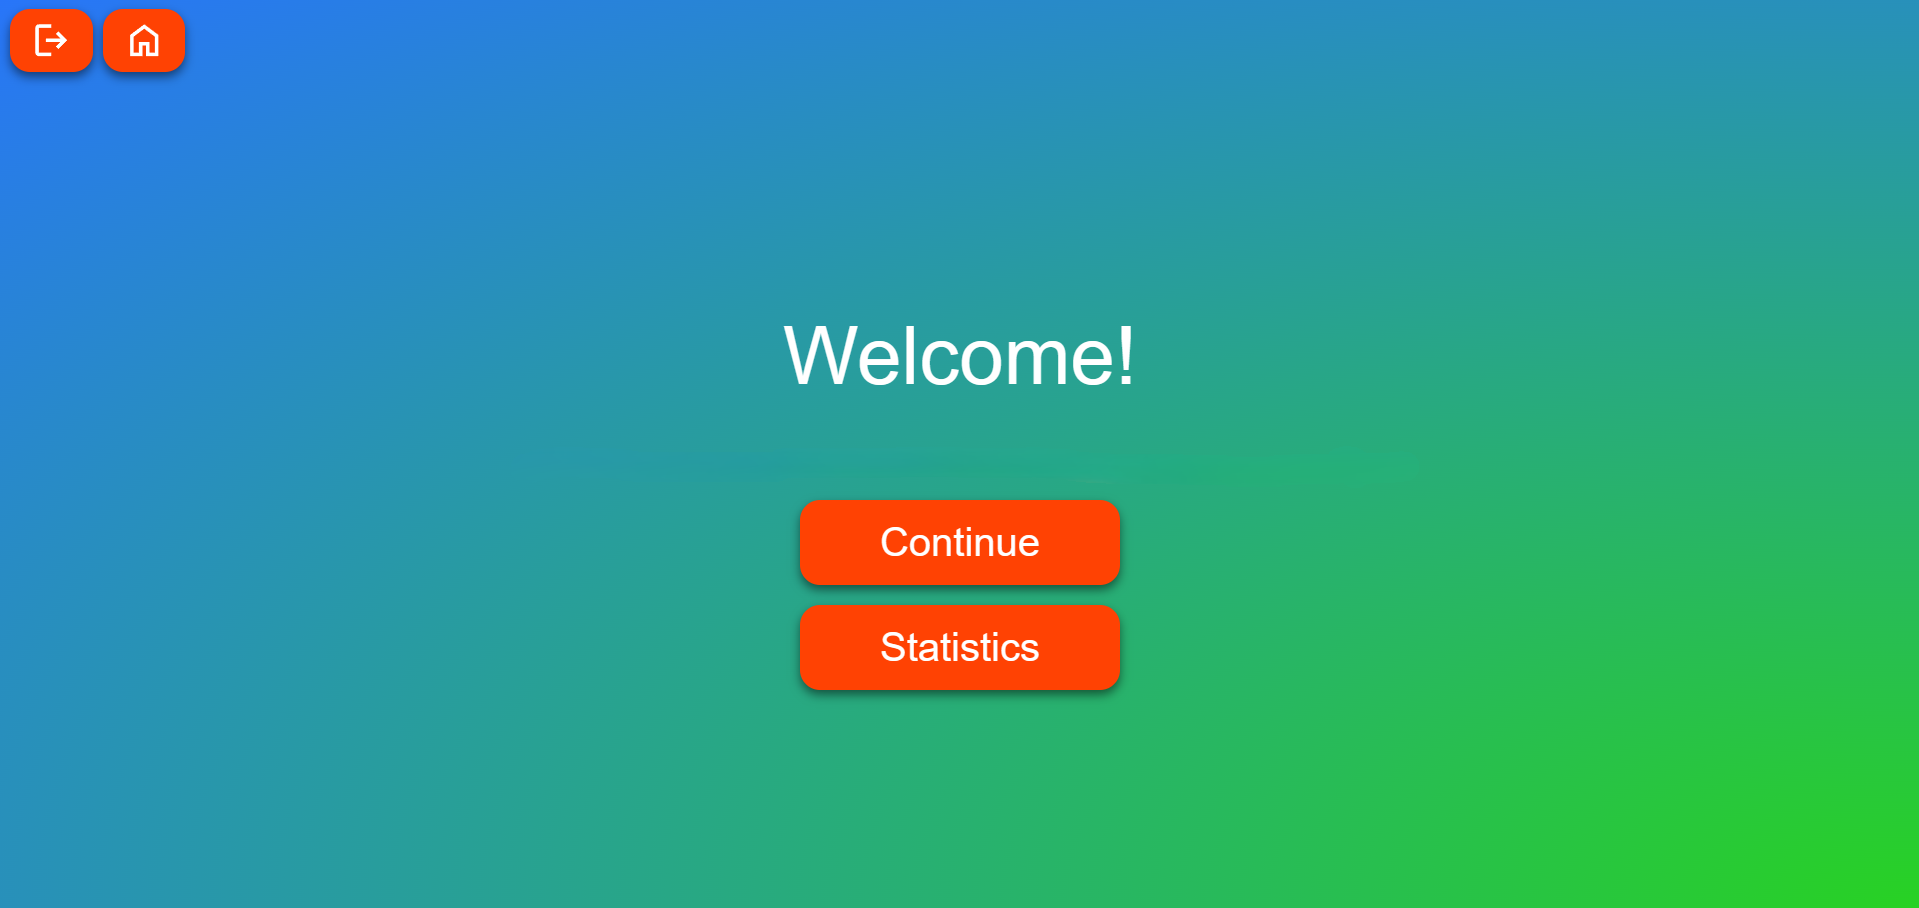
\includegraphics[width=1\linewidth]{img/Menu.png}
    \caption{\textlatin{Menu Page}}
\end{figure}

\begin{itemize}
    \item Παρακάτω βλέπουμε τα κεφάλαια της θεωρίας (\textlatin{\textbf{History, Geography, Culture}}). Ο μαθητής καλείται να τα διαβάσει και να τα αποστηθίσει όσο καλύτερα μπορεί, προκειμένου να βρίσκεται σε θέση να απαντήσει τα \textlatin{quizzes} που ακολουθούν, έπειτα από κάθε κεφάλαιο. Τα κεφάλαια χωρίζονται σε ενότητες με σκοπό την διευκόλυνση του μαθητή κατά την διάρκεια της εκμάθησης τους.
\end{itemize}
\begin{figure}[H]
     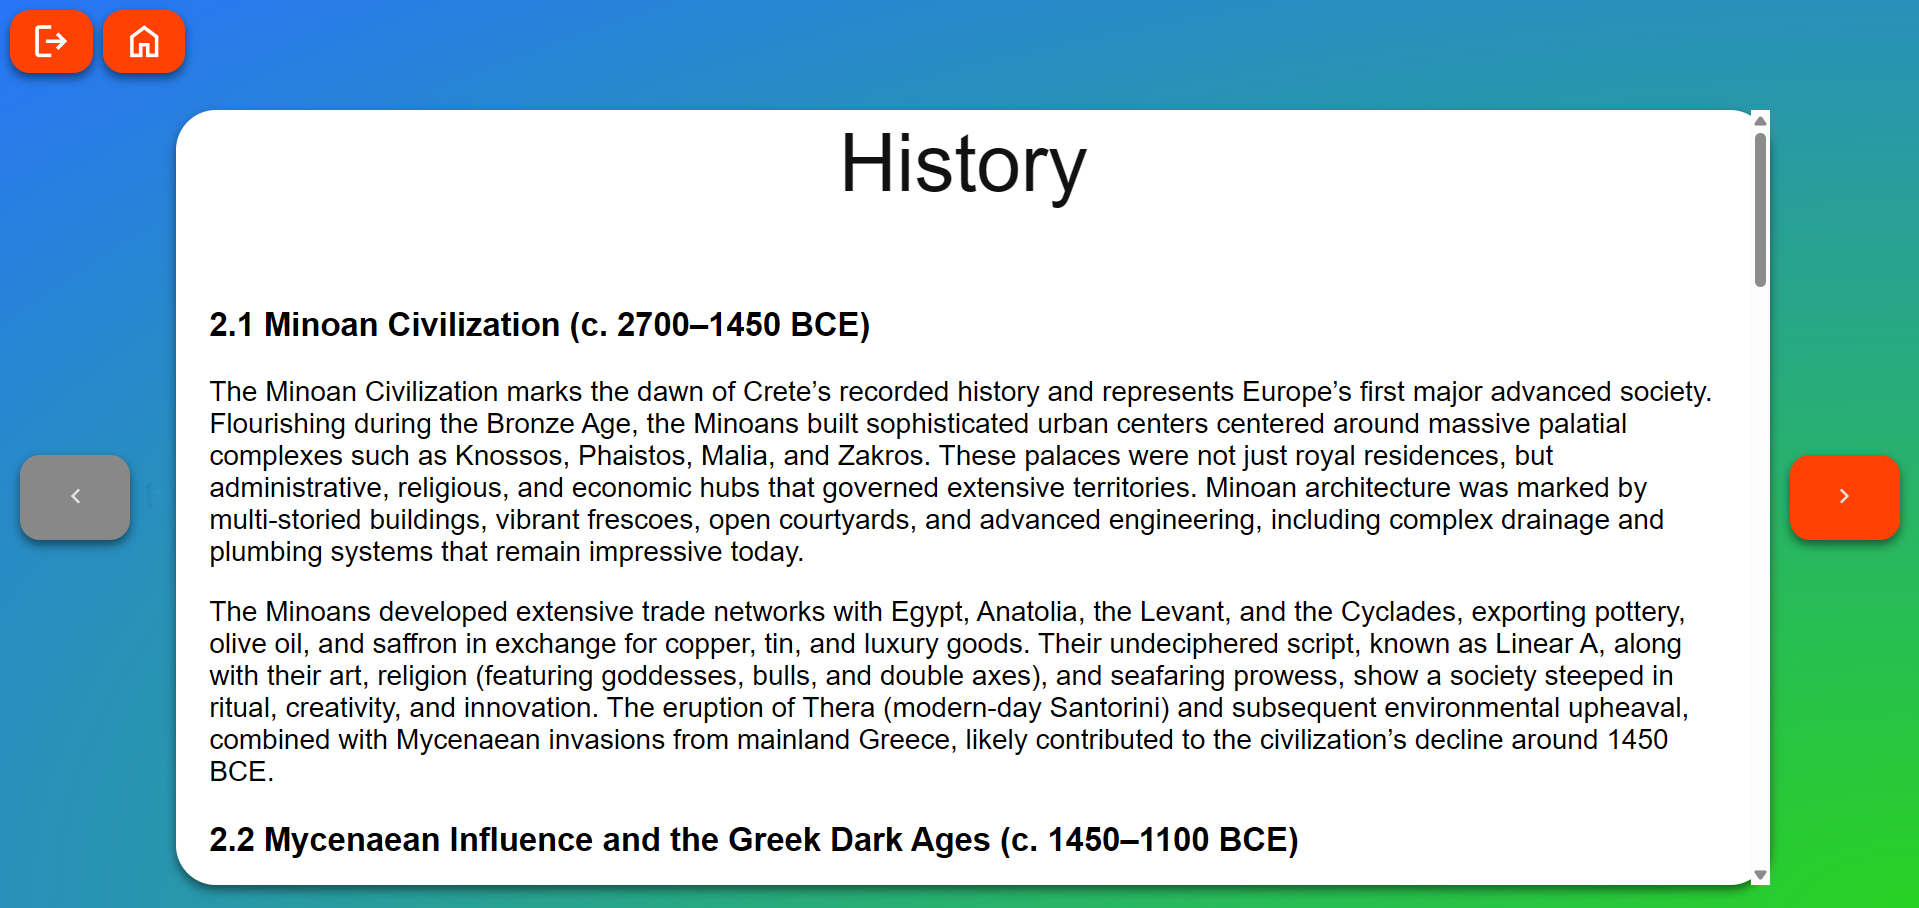
\includegraphics[width=0.5\linewidth]{img/Theory-History.png}
     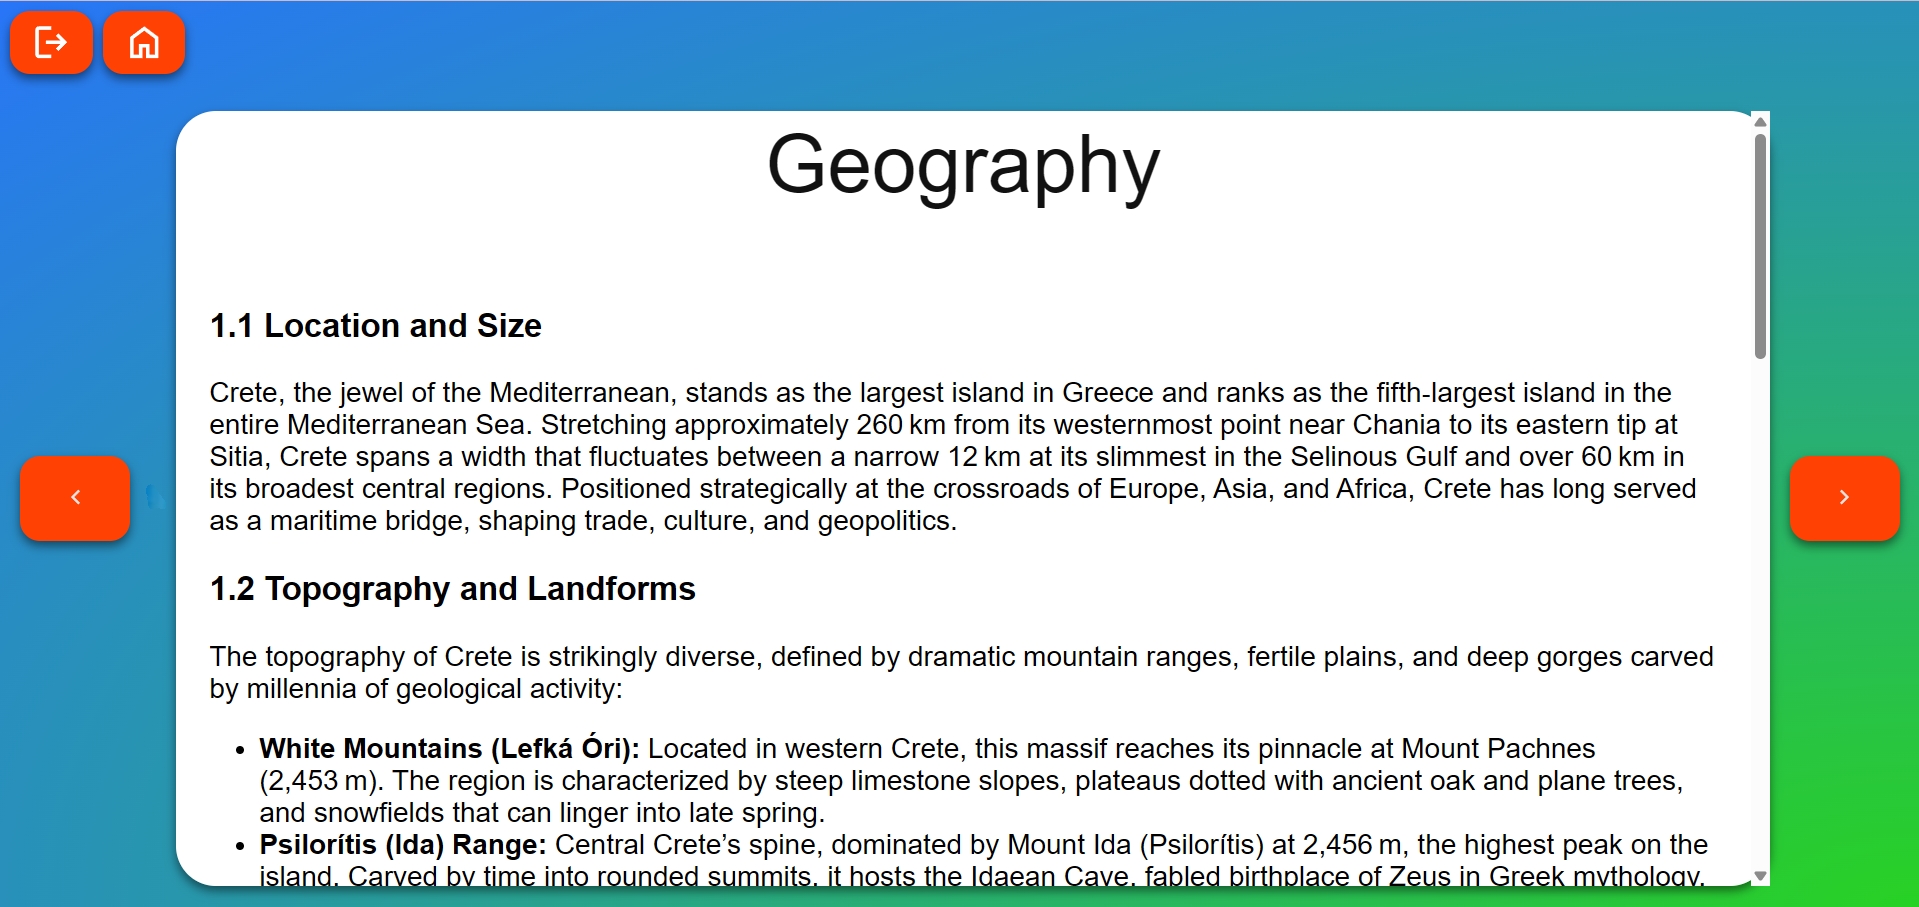
\includegraphics[width=0.5\linewidth]{img/Theory-Geography.png}
\end{figure}
\begin{figure}[H]
    \centering
    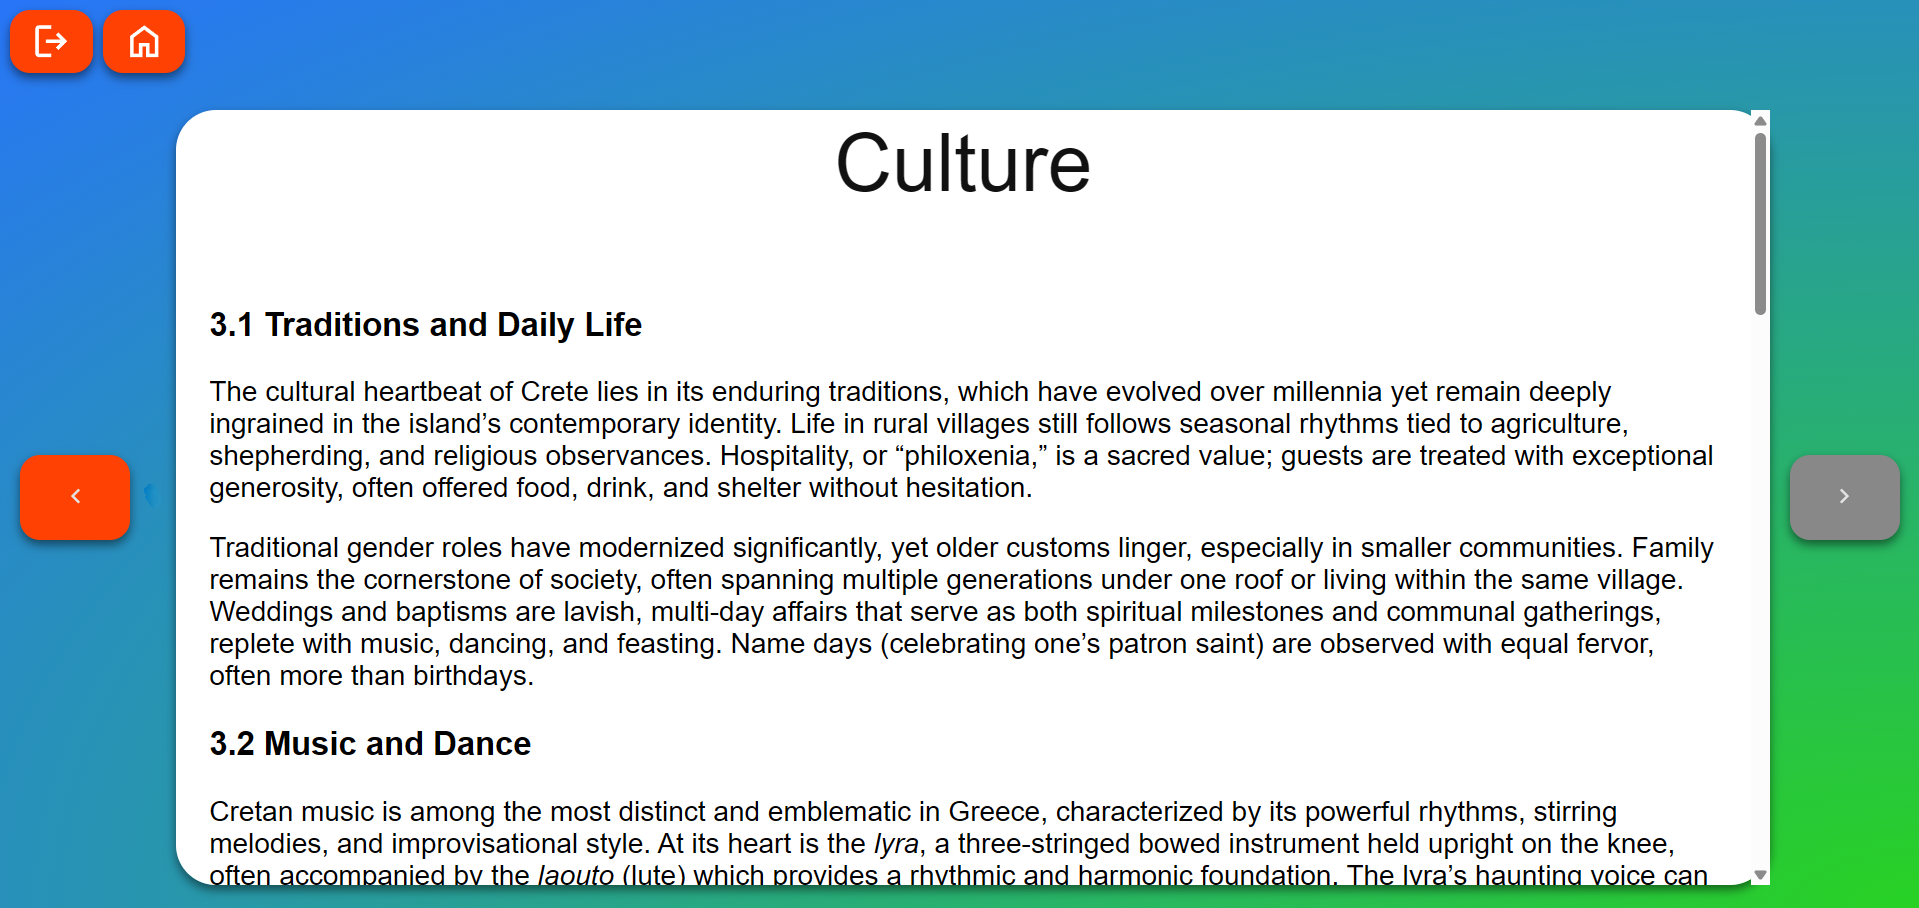
\includegraphics[width=0.5\linewidth]{img/Theory-Culture.png}
    \caption{\textlatin{Theory Chapters Page}}
\end{figure}

\begin{itemize}
    \item Στο τέλος κάθε κεφαλαίου θεωρίας, ο χρήστης θα βρει ένα \textbf{κουμπί \textlatin{"Take the Quiz"}} το οποίο θα τον οδηγήσει στο αντίστοιχο \textlatin{\textbf{quiz}} γνώσεων του συγκεκριμένου κεφαλαίου που βρίσκεται και ολοκλήρωσε. (Κάθε κεφάλαιο έχει από ένα \textlatin{quiz} 15 ερωτήσεων, άρα συνολικά έχουμε 3 \textlatin{quizzes} και 45 διαφορετικές ερωτήσεις).
\end{itemize}
\begin{figure}[H]
    \centering
    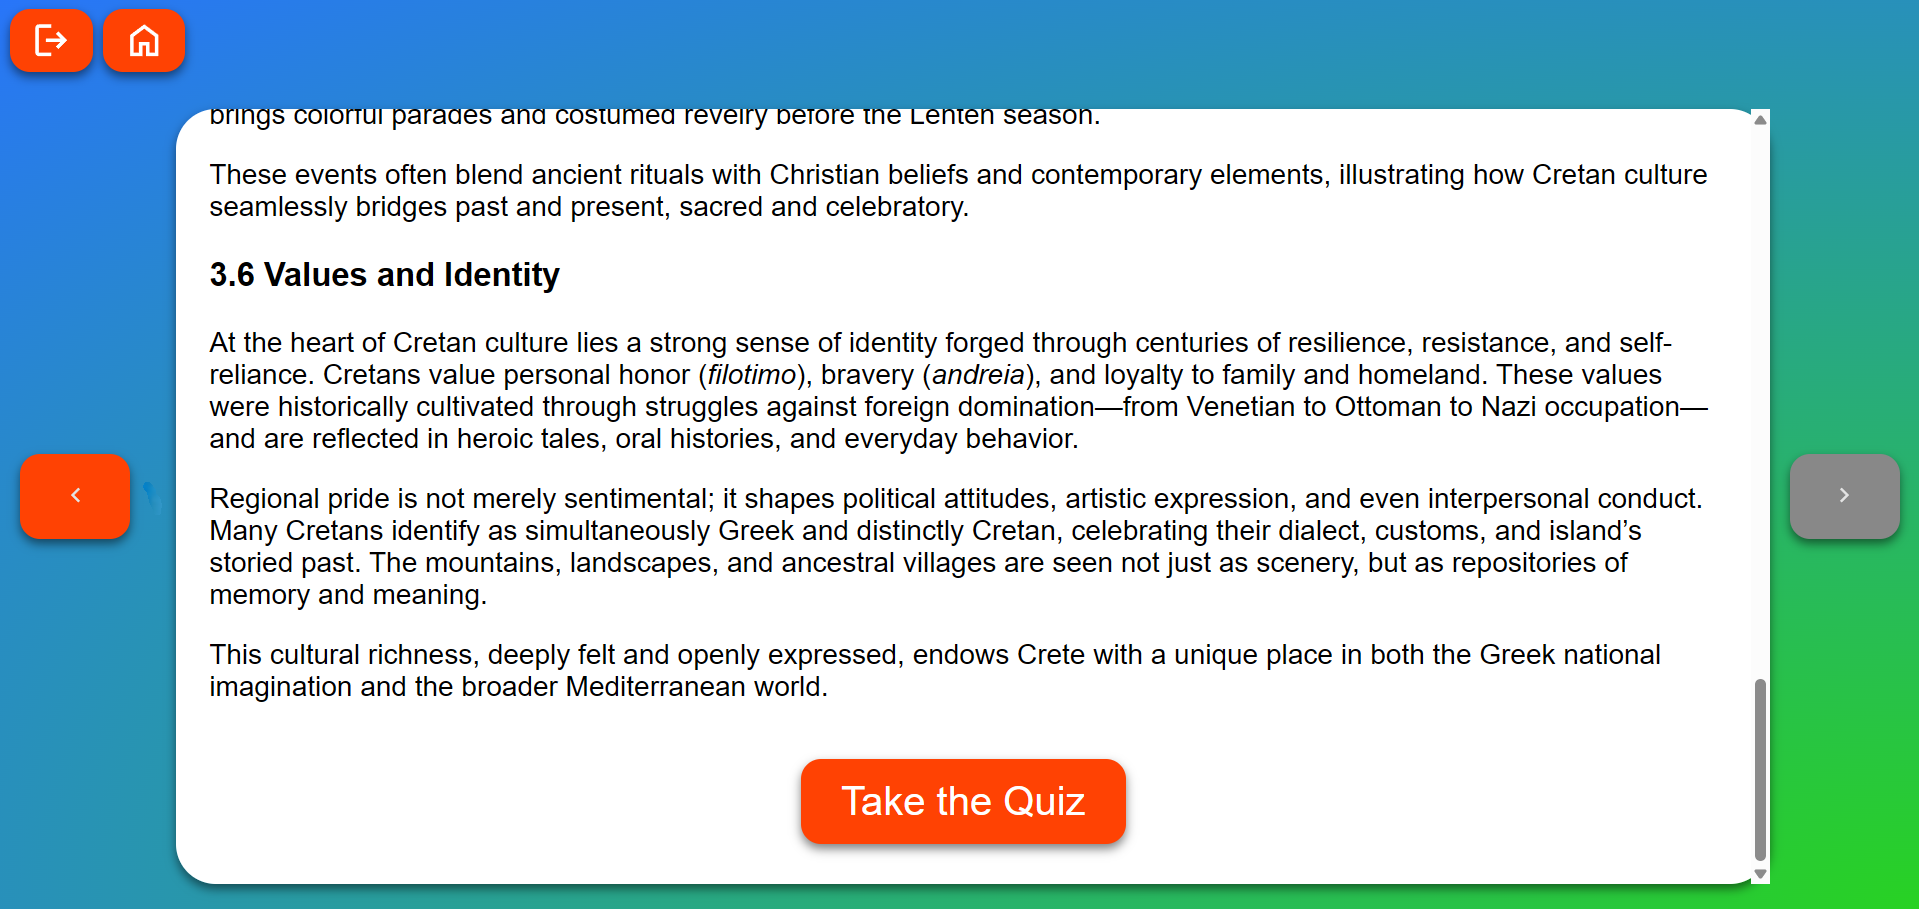
\includegraphics[width=1\linewidth]{img/Theory-TestButton.png}
    \caption{\textlatin{Theory Page-Quiz Button}}
\end{figure}

\begin{itemize}
    \item Αφού ο μαθητής έχει τελειώσει και απαντήσει όλες της ερωτήσεις των τριών κεφαλαίων, τελευταίο βήμα είναι να κάνει το τελικό, επαναληπτικό διαγώνισμα (\textlatin{\textbf{Exam}}), ειδικά προσαρμοσμένο πάνω στις γνώσεις, στις αδυναμίες και στις ικανότητες του κάθε μαθητή.
\end{itemize}
(φωτογραφία όταν τελειώσει)

\begin{itemize}
    \item Βέβαια, πριν το τελικό \textlatin{Exam}, θα προτείνεται στον μαθητή \textbf{έξτρα προσαρμοσμένο υλικό (\textlatin{Review})}, σύμφωνα με τις επιδόσεις του στα \textlatin{Quizzes}, εάν αυτό κρίνεται απαραίτητο (δηλαδή εάν το σκορ του μαθητή είναι χαμηλό).
\end{itemize}
\begin{figure}[H]
    \centering
    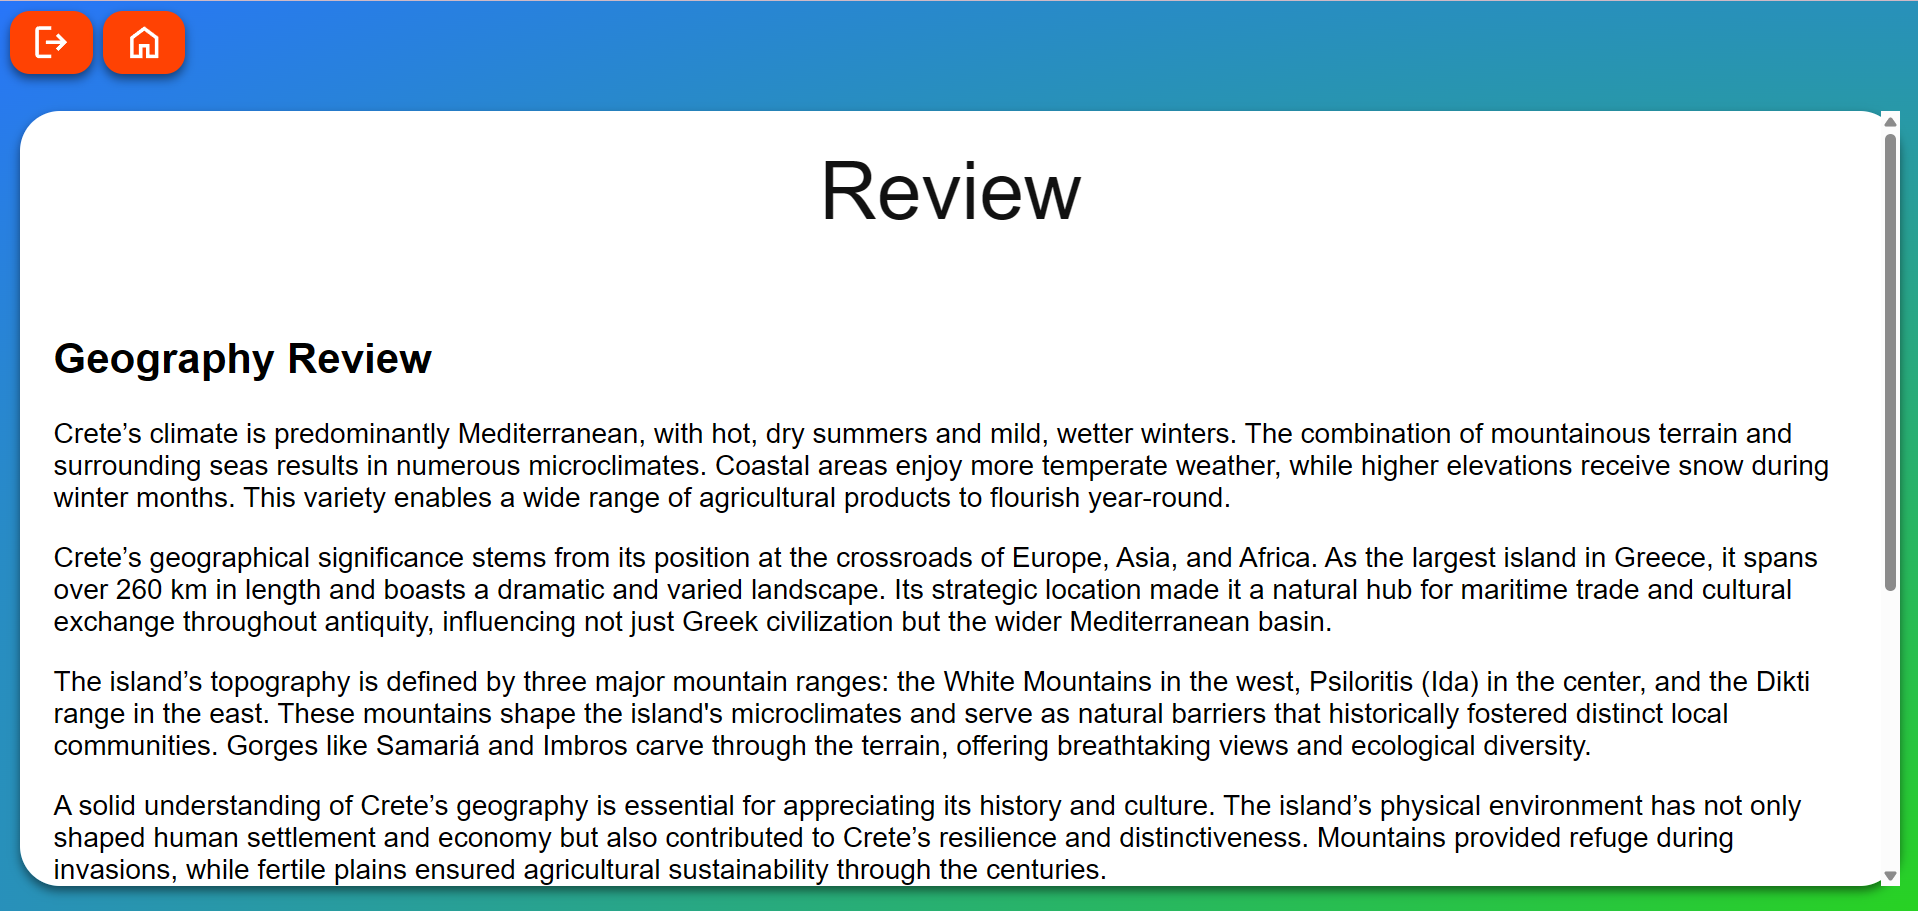
\includegraphics[width=1\linewidth]{img/Review.png}
    \caption{\textlatin{Review Page}}
\end{figure}



\begin{itemize}
    \item Ο μαθητής, θα έχει επίσης την δυνατότητα, να επισκέπτεται όσες φορές θέλει το κομμάτι της θεωρίας που επιθυμεί να επαναλάβει, έτσι ώστε να μάθει σε μεγαλύτερο βάθος και να προσαρμοστεί όσο καλύτερα γίνεται στα κεφάλαια μέσω \textlatin{\textbf{Chapters}}. Ακόμα, θα μπορεί να δει πόσες και ποιες ερωτήσεις έχει απαντήσει σε κάθε ένα από τα κεφάλαια ώστε να έχει μία "καθαρή" εικόνα της προόδου του.
\end{itemize}
\begin{figure}[H]
    \centering
    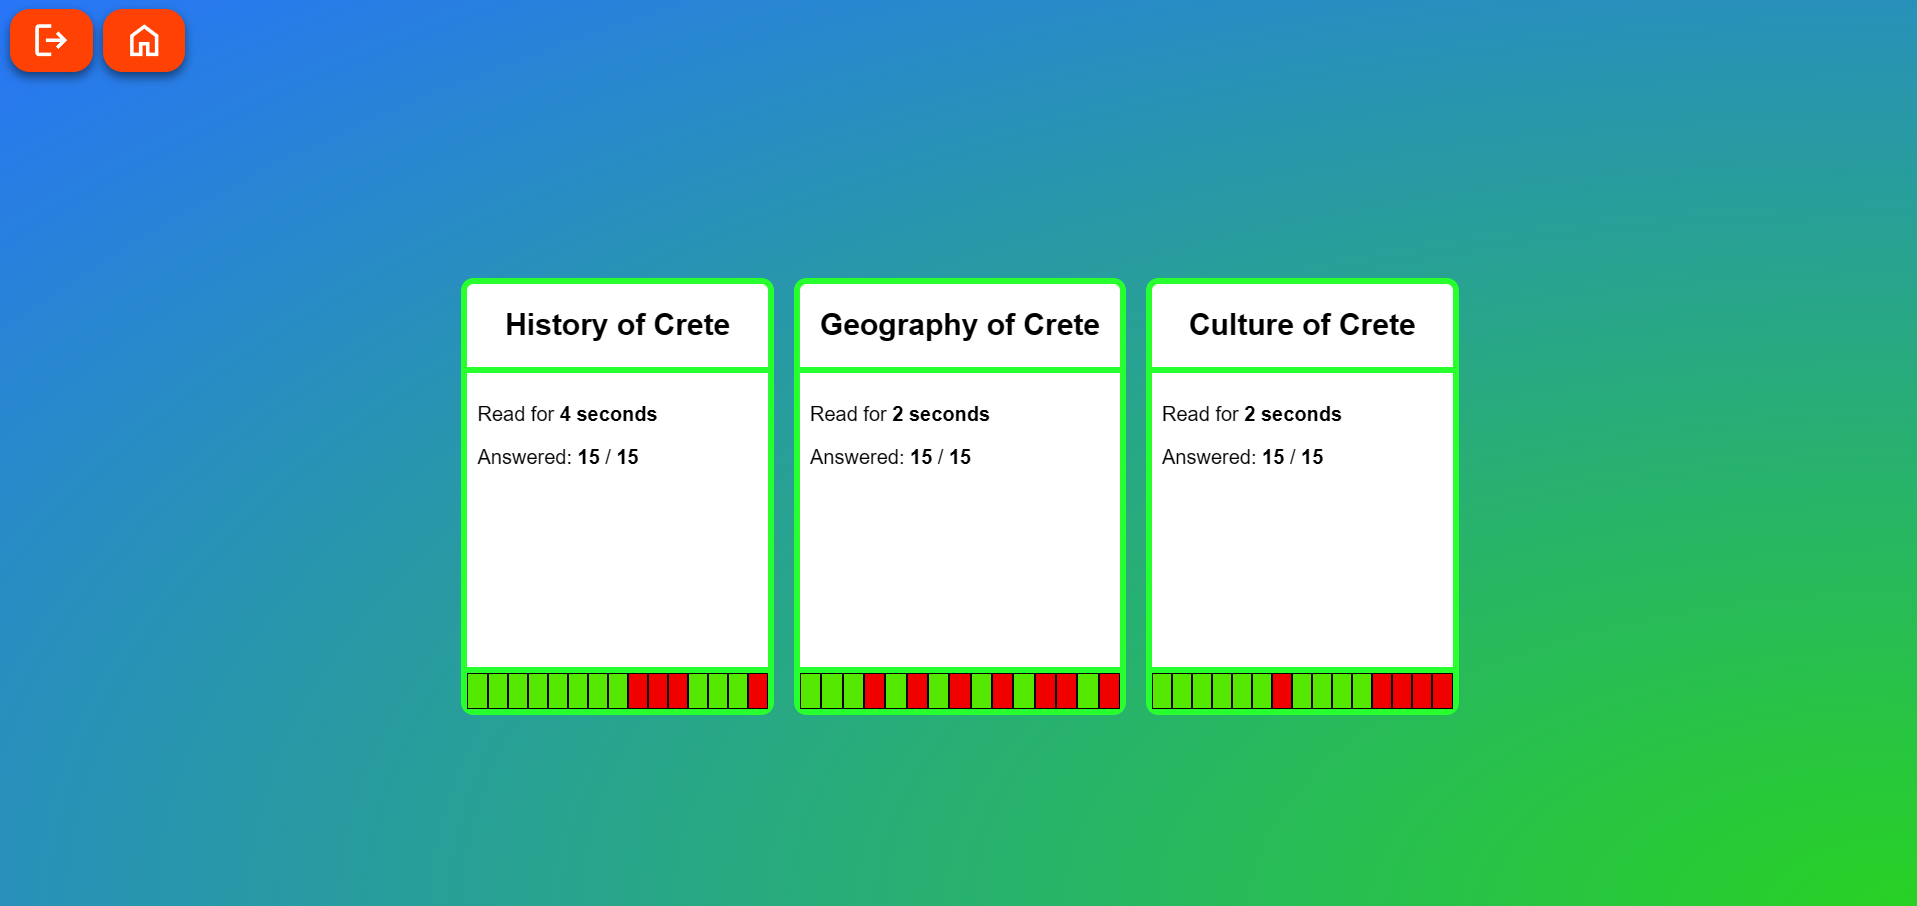
\includegraphics[width=1\linewidth]{img/Chapter-Progress.png}
    \caption{\textlatin{Chapter Progress Page}}
\end{figure}

\begin{itemize}
    \item Όσον αφορά το τμήμα των \textbf{Στατιστικών}, εκεί ο μαθητής θα έχει την δυνατότητα να ενημερώνεται για την πρόοδο του, τον χρόνο που καταναλώνει στα \textlatin{quizzes} και στο \textlatin{Exam} και συνεπώς να εντοπίζει τα πεδία στα οποία χρειάζεται περισσότερη μελέτη, με σκοπό την αυτοβελτίωσή του και την καλύτερη κατανόηση της ύλης. Τα γραφήματα θα στηρίζονται στην συνολική του εικόνα/ απόδοση, με γνώμονα κάθε κεφάλαιο ξεχωριστά και τέλος συγκεκριμένα για κάθε ερώτηση.
\end{itemize}
\begin{figure}[H]
    \centering
    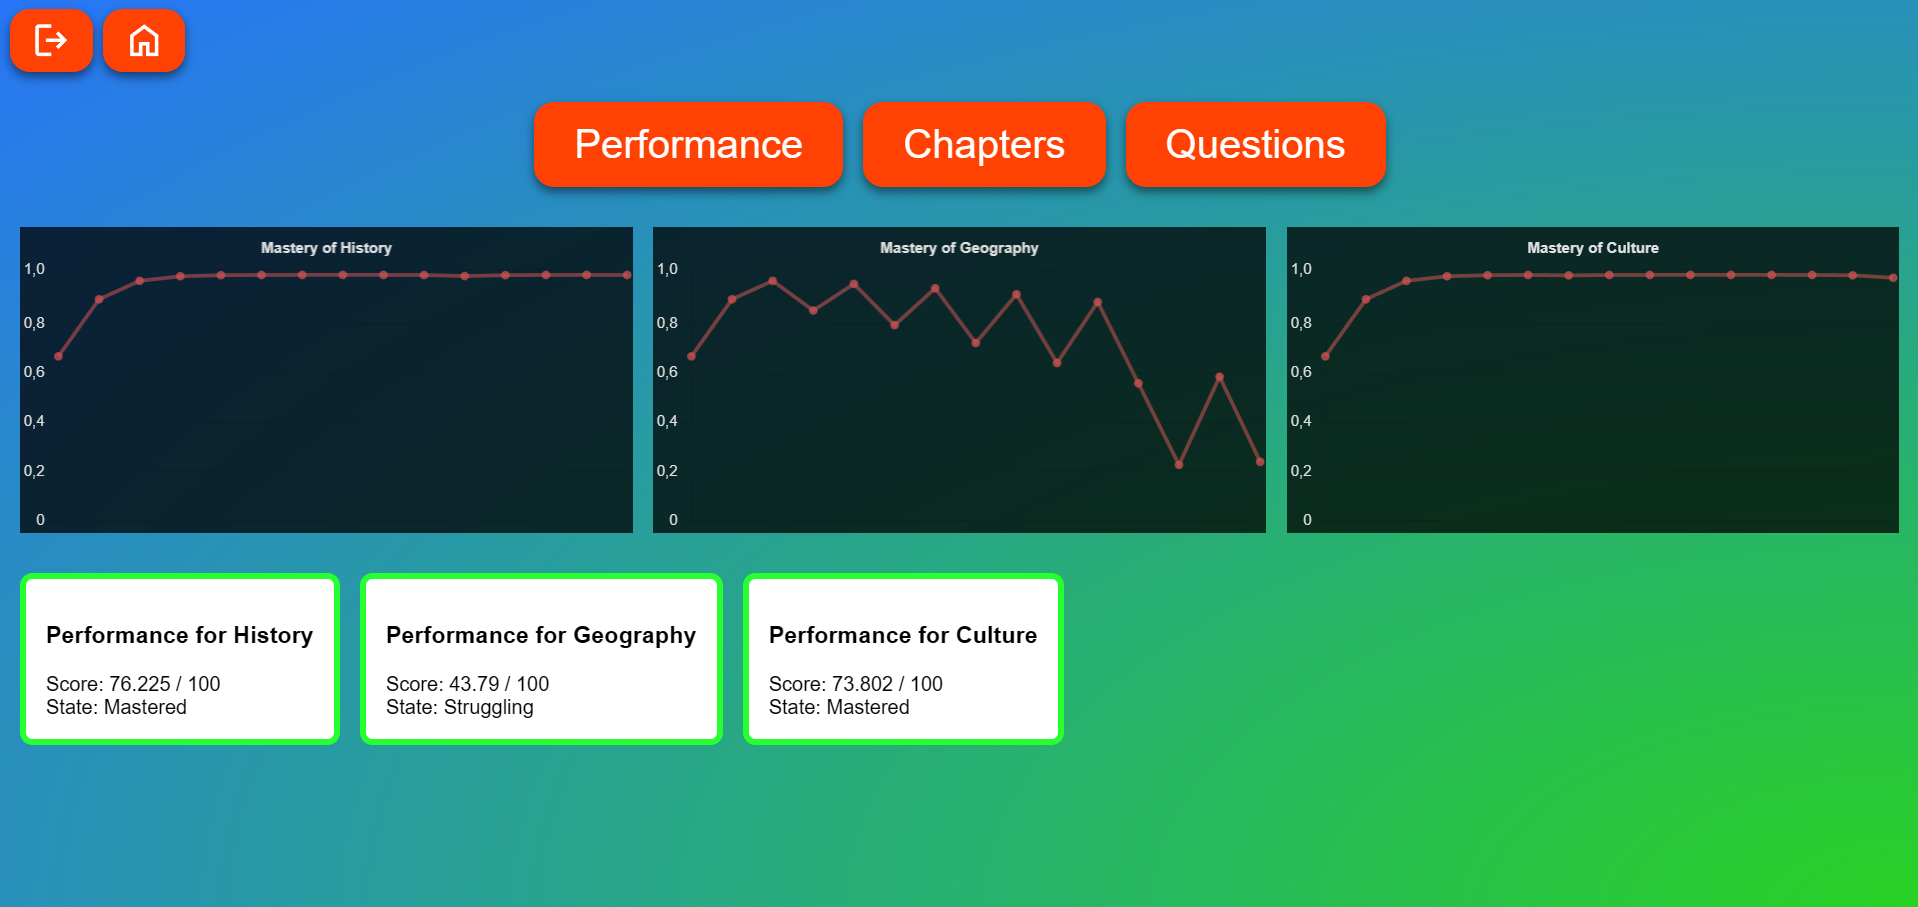
\includegraphics[width=0.5\linewidth]{img/Statistics.png}
    \caption{\textlatin{Statistics Page (Performance}}
\end{figure}
\begin{figure}[H]
    \centering
    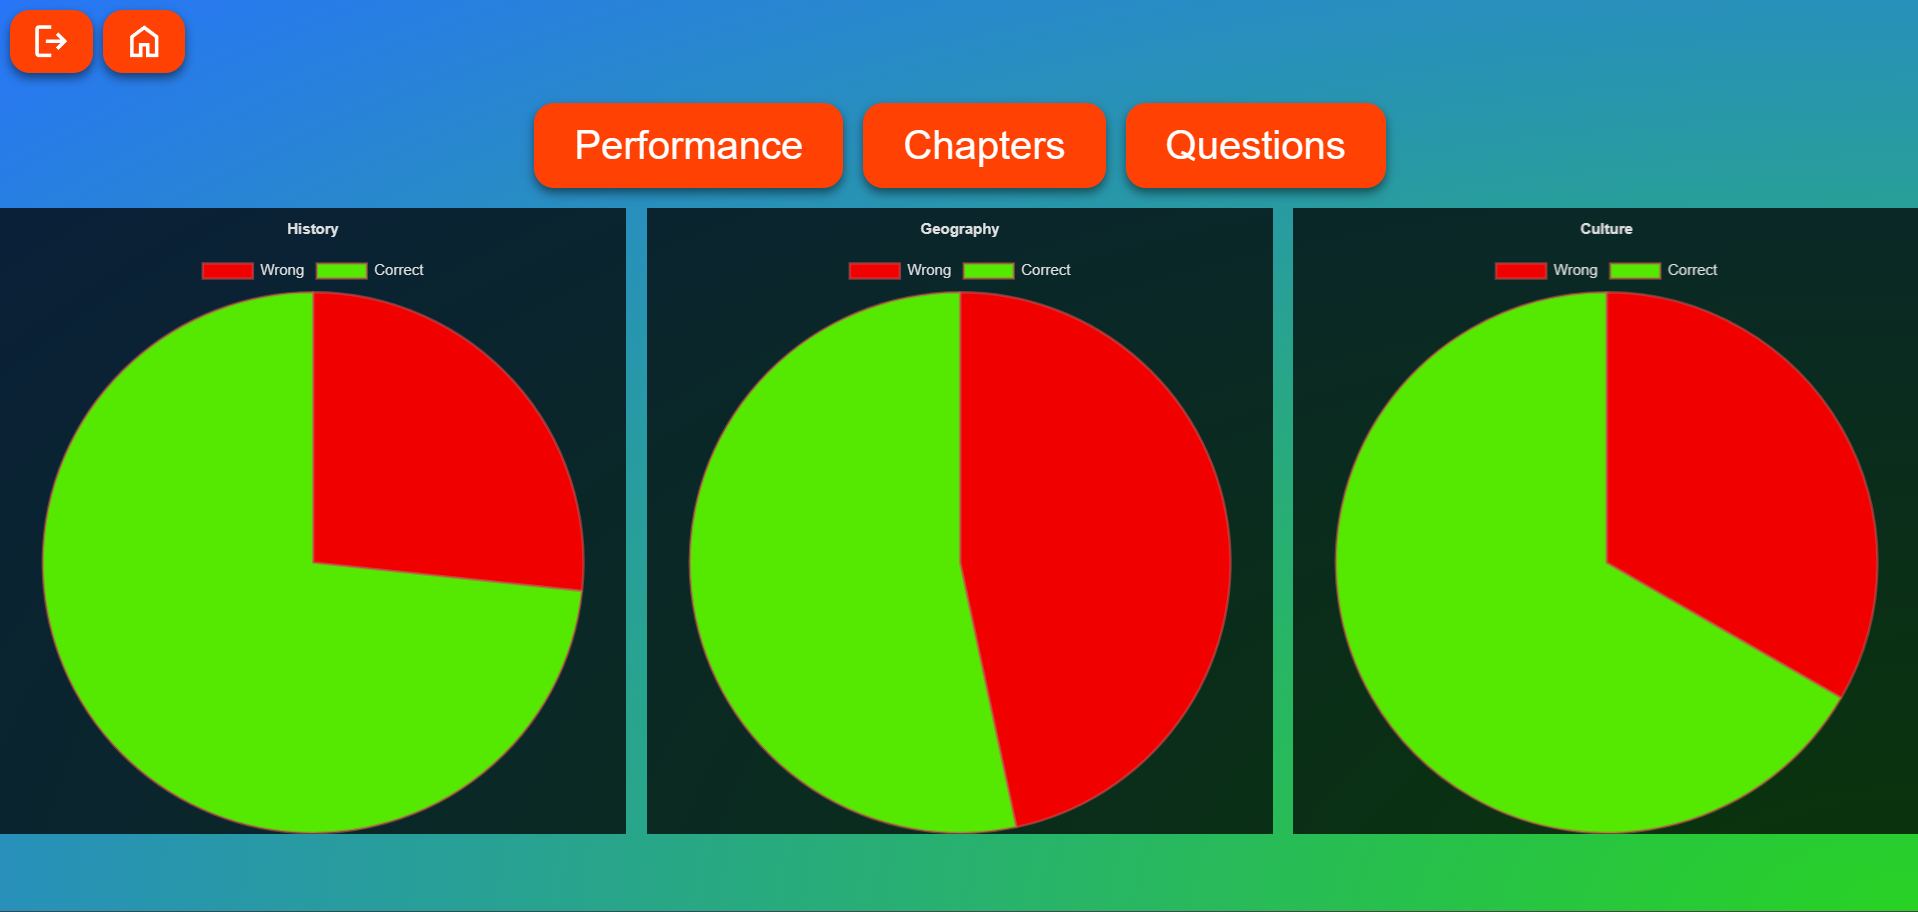
\includegraphics[width=0.5\linewidth]{img/Statistics-Quests.png}
    \caption{\textlatin{Statistics Page (Questions)}}
\end{figure}